\chapterauthor{Alan Gray and Kevin Stratford}{EPCC, The University of Edinburgh}

\chapter{Ludwig}

%\putbib[biblio]


\section{Introduction}
The lattice Boltzmann (LB) method (for an overview see, e.g.,
\cite{succi-book}) has become a popular approach to a variety of fluid
dynamics problems.  It provides a way to solve the incompressible,
isothermal Navier-Stokes equations and has the attractive features of
being both explicit in time and local in space. This makes the LB
method well-suited to parallel computation. Many efficient parallel
implementations of the LB method have been undertaken, typically using
a combination of distributed domain decomposition and the Message
Passing Interface MPI \cite{mpi-standard}. However, the potential
performance benefits offered by GPUs has motivated a new `mixed-mode'
approach to address verly large problems. Here, fine-grained
parallelism is implemented on the GPU, while MPI is reserved for
larger-scale parallelism.  This mixed mode is of increasing interest
to application programmers as many supercomputing services are moving
toward clusters of GPU accelerated nodes.

The \textit{Ludwig} code \cite{desplat} is a LB package developed
specifically for complex fluid problems, for example mixtures,
surfactants, liquid crystals, and particle
suspensions~\cite{aidun2010}.  In this chapter we present the steps
required to allow Ludwig to efficiently exploit many NVIDIA GPUs in
parallel.  We show that Ludwig scales excellently to at least the
thousand GPU level (the largest resource available at the time of
writing) with indications that the code will scale to much larger
systems as they come on-line. We first consider the problem of a
binary fluid mixture (e.g., oil and water) modelled using the LB
approach, and we go on to describe how we deal with the complexities
arising when colloidal particles are introduced to interact with the
fluid.

In Section \ref{ch14:sec:background} we give background details to
introduce the the methods being employed. In Section
\ref{ch14:sec:singlegpu}, we describe the adaptations made to Ludwig
to allow it to efficiently exploit the GPU architecture. In Section
\ref{ch14:sec:singlegpu}, we extend this description to the work
required to allow exploitation of many GPUs in parallel. We present
performance and scaling results, for the binary fluid case, in Section
\ref{ch14:sec:performance}, before going, in Section
\ref{ch14:sec:particles}, to describe how we minimise the overheads
involved with introducing colloidal particles.



\section{Background}\label{ch14:sec:background}

\begin{figure}[!t]
\centering
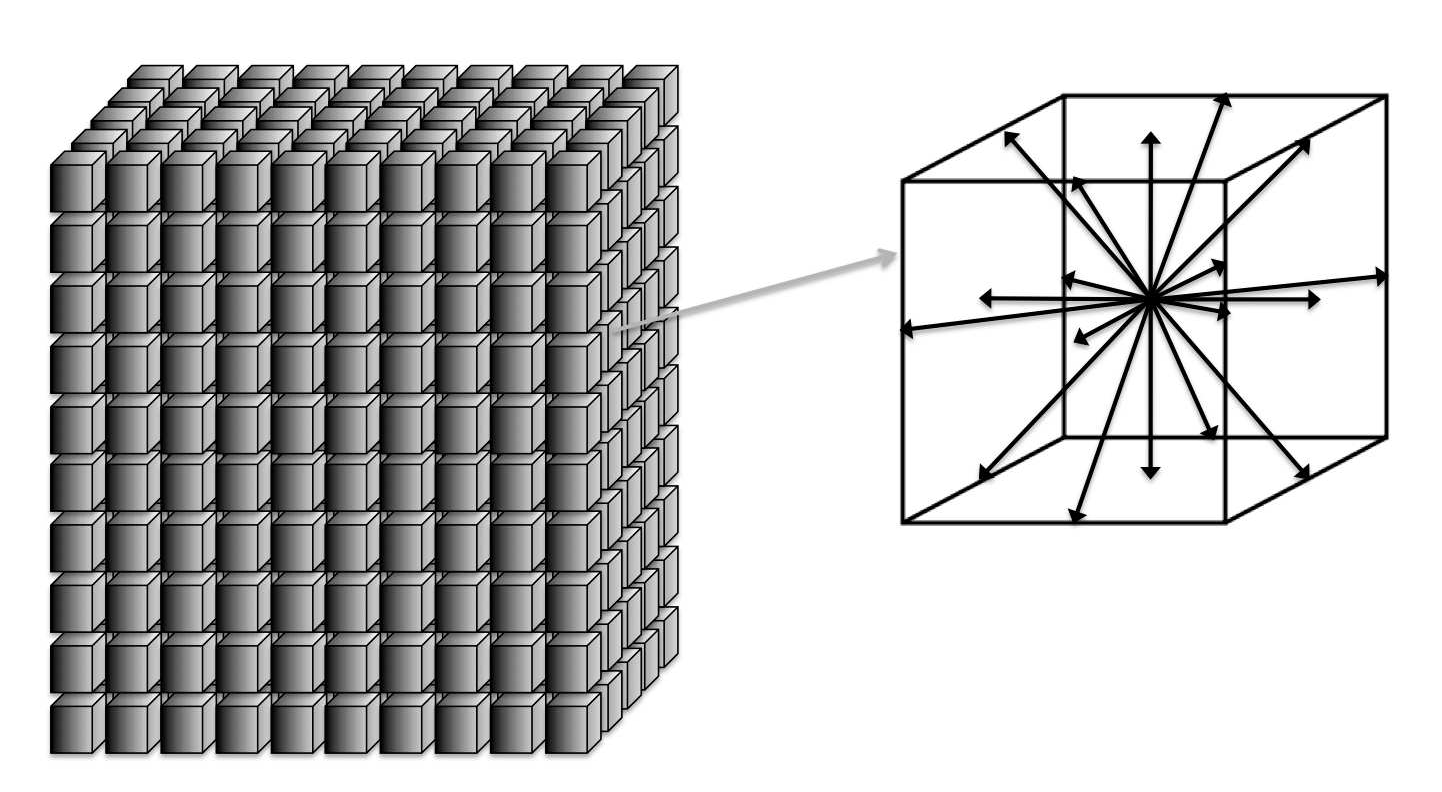
\includegraphics[width=12cm]{Chapters/chapter14/figures/basiclattice}
\caption{The lattice Boltzmann approach discritises space into a 3D lattice (left). The fluid is represented at each lattice site (right), by the {\it distribution} vector: each component corresponding to a specific velocity direction. Here we are interested in the {\it D3Q19} model, in which there are 3 spatial directions and 19 velocity components (including a zero component).}
\label{ch14:fig:basiclattice}
\end{figure}

A symmetric binary fluid, in which both components have the same
density and viscosity, may be described by introducing a composition
variable or \textit{order parameter} $\phi(\mathbf{r})$. This is
a function of position $\mathbf{r}$ and describes the relative
proportions of the two fluids present locally. To describe the
thermodynamics of the system it is possible to write down a
\textit{free energy} which is a functional of the order parameter.
The equation of motion for $\phi$ is then
\begin{equation}
\partial_t \phi + \mathbf{\nabla}.(\mathbf{u}\phi) = 
- \mathbf{\nabla} . (M \mathbf{\nabla}\mu),
\label{cahn-hilliard}
\end{equation}
where $\mu$ is the chemical potential related to the functional derivative
of the free energy, and $M$ is a mobility. This couples
to the fluid velocity field $\mathbf{u}(\mathbf{r})$, whose evolution
obeys the Navier-Stokes equations describing the conservation of mass
(or density $\rho$) and momentum
\begin{equation}
\rho  [ \partial_t \mathbf{u} + (\mathbf{u}.\mathbf{\nabla})\mathbf{u} ]
= -\nabla p + \eta \nabla^2 \mathbf{u} + \mathbf{f}(\mathbf{r}),
\end{equation}
where $p$ is the isotropic pressure and $\eta$ is the viscosity.
A force density
$\mathbf{f}(\mathbf{r})$  describes the force exerted by a
curved fluid interface on the fluid. It is sufficient to note
here that this force depends locally on the order parameter and its
derivatives $\nabla\phi$ and $\nabla^2 \phi$. For a full
description the interested reader is referred to, e.g.,
\cite{bray1994,kendon2001}.

The LB approach makes use of a regular 3-dimensional
lattice (see Figure \ref{ch14:fig:basiclattice}) with discrete spacing $\Delta r$. It also makes use of a
discrete velocity space $\mathbf{c}_i$, where the $\mathbf{c}_i$
are chosen to capture the correct symmetries of the Navier-Stokes
equations. A typical choice, used here, is the so-called D3Q19
basis in three dimensions where there is one velocity such that
$\mathbf{c} \Delta t$ is zero, along with six extending to the nearest
neighbour
lattice sites, and twelve extending to the next-nearest neighbour sites
($\Delta t$ being the discrete time step). The fundamental object
in LB is then the distribution function $f_i (\mathbf{r};t)$ whose
moments are related to the local hydrodynamic quantities: the fluid
density, momentum, and stress. The time evolution of the distribution
function is described by a discrete Boltzmann equation
\begin{equation}
f_i(\mathbf{r} + \mathbf{c}_i \Delta t; t) - f_i(\mathbf{r}; t) 
= - {\cal L}_{ij} f_j(\mathbf{r};t).
\end{equation}
It is convenient to think of this in two stages. First, the right hand
side represents the action of a collision operator ${\cal L}_{ij}$,
which is local to each lattice site and relaxes the distribution toward
a local equilibrium at a rate ultimately related to the fluid viscosity.
Second, the left hand side represents a propagation step (sometimes referred
to as streaming step), in which each element $i$ of the distribution is
displaced $\mathbf{c}_i \Delta t$, i.e., one lattice spacing in the
appropriate direction per discrete time step. 

Computationally, we store a vector of 19 double precision floating
point values at each lattice site for the distribution function $f_i$.
The collision operation, which is local at each lattice site, may be
thought of as follows. The matrix-vector multiplication $L_{ji}f_i$ is
used to transform the distributions into the hydrodynamic quantities,
where $L_{ij}$ is a constant 19x19 matrix related to the choice of
$\mathbf{c}_i$. The non-conserved hydrodynamic quantities are then
relaxed toward their (known) equilibrium values, and are transformed
back to new post-collision distributions via the inverse transformation
$L^{-1}_{ij}$. This gives rise to the need for a minimum of 2x19$^2$
floating point multiplications per lattice site. In contrast, the
propagation stage consists solely of moving the distribution values
between lattice sites, and involves no floating point operations.

To represent the composition variable, we introduce a second distribution
function $g_i (\mathbf{r};t)$ whose first moment is $\phi$, second moment
is the order parameter flux, and so on \cite{swift1996}.
The time evolution of this second distribution follows an analogous
collision and propagation process to that described for $f_i$, and
so provides a solution to Eq.~\ref{cahn-hilliard} \cite{stratford-jsp2005}.

\begin{figure}[!t]
\centering
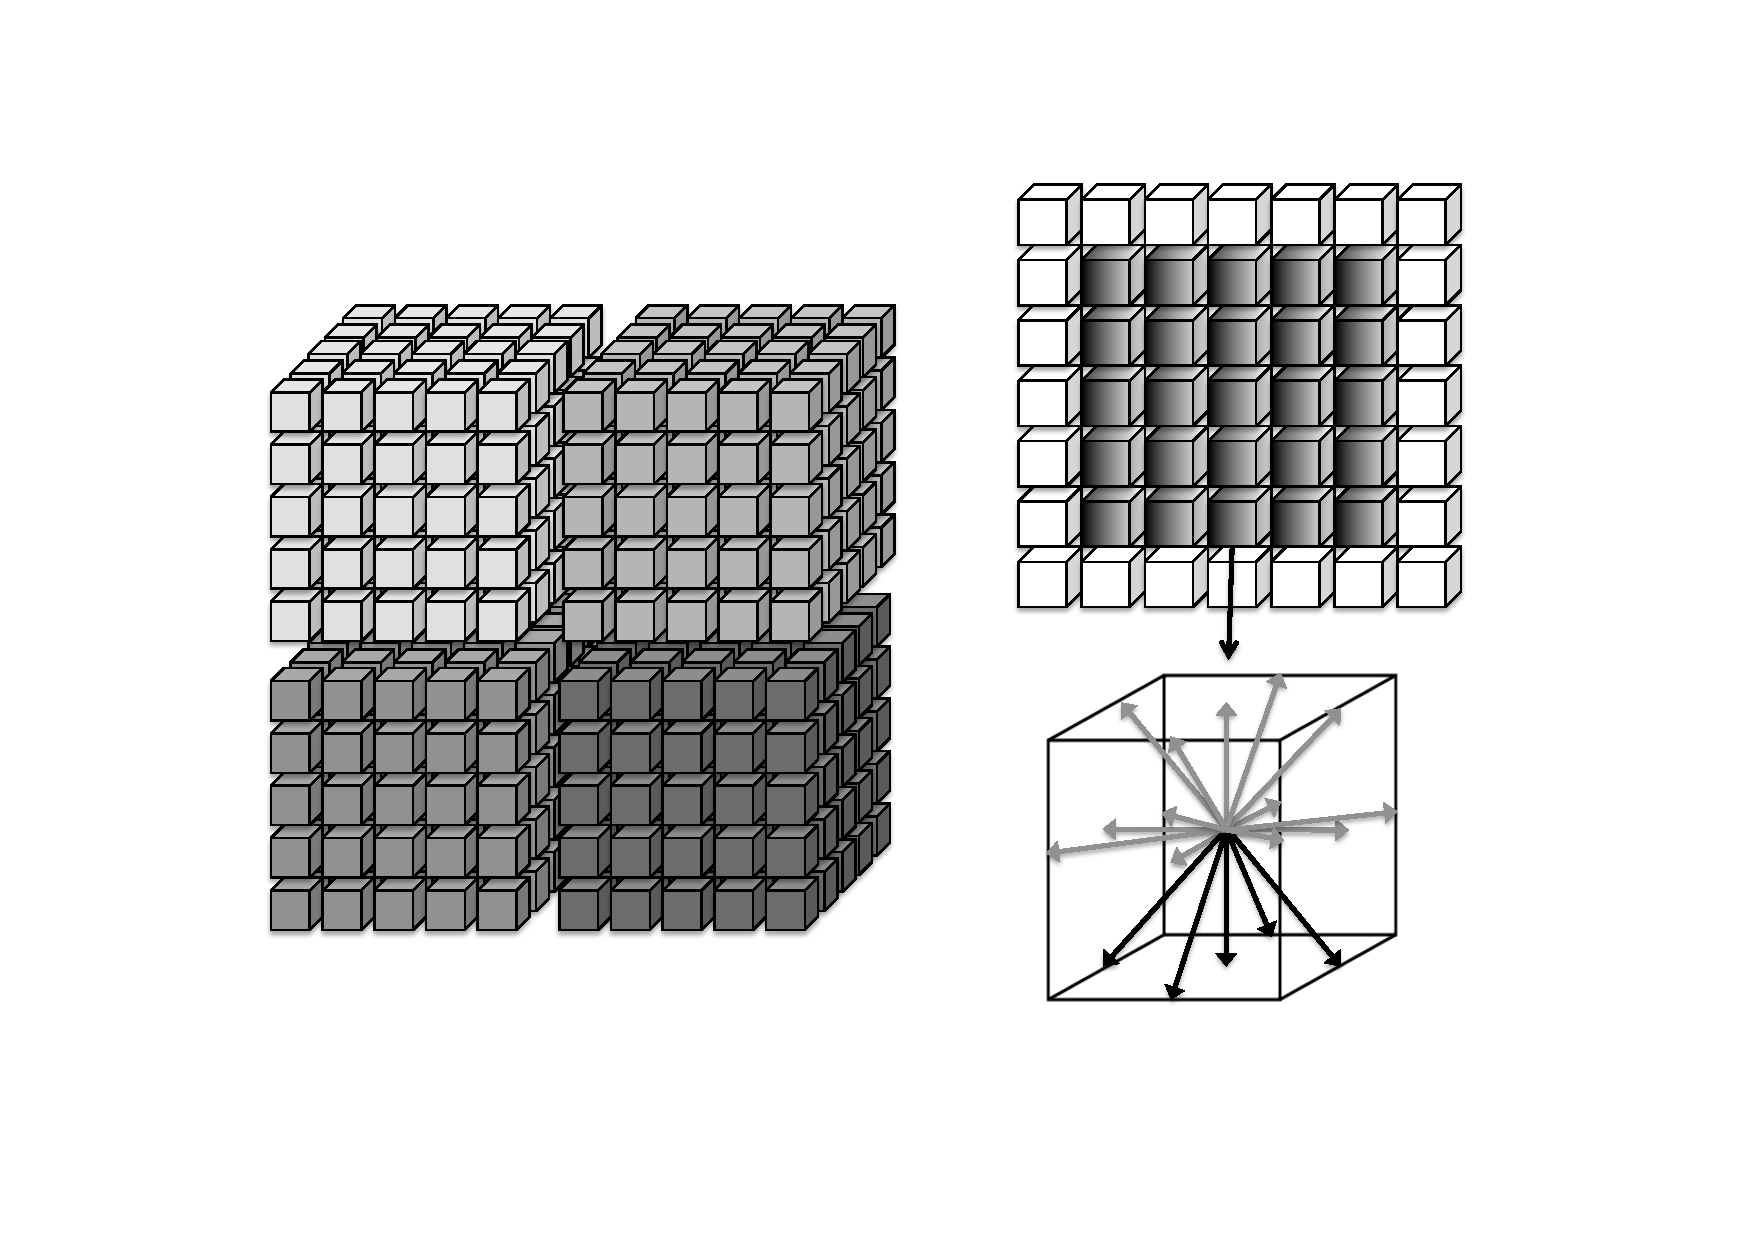
\includegraphics[width=12cm]{Chapters/chapter14/figures/decomphalo}
\caption{Left: the lattice is decomposed between MPI tasks. For clarity we show a 2D decomposition of a 3D lattice, but in practice we decompose in all 3 dimensions. Halo cells are added to each sudomain, as shown on the right for a single slice, which store data retrieved from remote neighbours in the halo exchange.}
\label{ch14:fig:decomphalo}
\end{figure}


As illustrated in Figure \ref{ch14:fig:decomphalo}, Ludwig is
parallelized (across CPU cores) using a regular 3D domain decomposition
where communications are performed via message passing using MPI.  We
note that while the collision is local for $f_i$, computation of the
force terms requires the evaluation of the derivatives of $\phi$ via a
standard finite different stencil.  This gives rise to the need for a
halo exchange involving the scalar $\phi$ before the collision.
Before the propagation stage, a halo exchange in both $f_i$ and $g_i$
is required.

For a 3D halo exchange, 2D planes of data are exchanged in each of the
positive and negative directions, for each of the 3 dimensions, i.e. 6
planes are sent and received by each process.  For the CPU version of
Ludwig, MPI datatype functionality is used to designate these planes.
The $\phi$ halo exchange involves scalar values at each site, whereas
the distribution halo exchange involves a higher volume of data since
we must transfer multiple components of each velocity vector. However
the number of velocity components included in a given transfer can be
filtered from 19 to 5 (for D3Q19), since only those elements
propagating outward from a local domain play a role in the propagation
stage. The specific components required depend on the direction of
transfer, and again MPI datatype functionality is used to designate
this.



\section{GPU Implementation}\label{ch14:sec:singlegpu}


In this section we describe the methods used to enable Ludwig
for the GPU architecture and describe some key optimizations that
significantly enhance performance.

To ensure that \textit{Ludwig} remains suitable for CPU-based systems,
we augment rather than modify the original code. All new GPU-related
functionality are implemented in an additive manner, mirroring the
modular structure of the original code. The new GPU modules have
interfaces similar to the original CPU functions, and the ability to
switch between versions is achieved at compile-time via C
pre-processing directives.  All GPU compute kernels are implemented using
CUDA.  Wrapper routines are developed to specify the
decomposition, invoke the CUDA kernels and perform the necessary data
management operations: the latter are facilitated through newly
developed modules for creation and destruction of device memory
structures, the copying of data between host and device, and where
necessary the packing and buffering of data.

The most important code section, in terms of performance, is the
collision stage. But it is important to offload all other
computational components of the timestep. Kernels with relatively low
computational demand, such as the propagation stage and operations
involving the order parameter, are also GPU enabled: this allows data
to remain resident on the GPU, and avoids expensive host-device data
transfer at each timestep (which would reduce the benefit of GPU
acceleration).  In order to port to the GPU in an incremental fashion,
while retaining the ability to test for correctness throughout the
process, we require a suite of data management functions. For each
data structure (such as the distribution, which we will use as an
example), we maintain a copy in both the CPU and GPU memory spaces.
Functions such as \verb+put_dist_on_gpu()+, and
\verb+get_dist_from_gpu()+, which abstract underlying CUDA
functionality, allow us to update the GPU copy from the host copy and
vice versa\footnote {Within the implementation of these functions we
  have to work around data encapsulation issues. In the code, the use
  of the file scope identifier \texttt{static} prevents direct access
  to data; instead access functions are provided.  For the GPU code,
  it was necessary to use these existing access functions to copy
  these data to equivalent arrays on the device (via temporary buffers
  on the host).  Within the CUDA kernel, the data access function
  calls are substituted with array accesses.  The process is reversed
  when encapsulated data needs to be transferred back to the host.}.
This makes it easy, in the function implementing the Ludwig timestep,
to switch between the CPU and GPU for different components in the
timestep: we can develop GPU functionality incrementally while
retaining a code that runs correctly (albeit slowly due to data
transfer overheads).  Once every component in the timestep is
GPU-enabled, then it becomes possible to move such data transfers
outside the timestep loop, and just use the GPU-resident versions
throughout the simulation.

To achieve optimal performance, it is vital to fully exploit
parallelism inherent to the NVIDIA architecture, particularly for
those matrix-vector operations within the dominant collision kernel. A
simplified schematic of a serial implementation of such a matrix-vector
operations is as follows:
{\footnotesize
\begin{verbatim}
// loop over lattice sites
for ( is = 0; is < N; is++){
  ...
  //load distribution from site-major structure
  for (i = 0; i < 19; i++)    
    f[i]=f_all[is][i]
  ...
  //perform matrix-vector multiplication  
  for (i = 0; i < 19; i++){    
    a[i] = 0.0;    
    for (j = 0; j < 19; j++){      
      a[i] += f[j]*L[i][j];   
    }
  }
  ...
}
\end{verbatim}
}
The GPU architecture features a hierarchy of parallelism. At the
lowest level, groups of 32 threads called {\it warps} operate in
lock-step on different data elements - this is SIMD style vector-level
parallelism. Multiple warps are combined into a thread block (in which
communication and synchronisation are possible), and multiple blocks can
run concurrently across the SMs in the GPU (with no communication or
synchronisation possible across blocks).  To decompose on the GPU, we
must choose which of the above loops to assign to which level of
parallelism.

There exists parallelism within the matrix-vector operation, but the
length of each {\it distribution} vector, at 19, is smaller than the
warp size and typical thread block sizes. So therefore we simply
decompose the loop over lattice sites to all levels of parallelism,
i.e.  we use a separate CUDA thread for every lattice site, and each
thread performs the full matrix-vector operation. We find that a block
size of 256 performs best: we decompose our lattice domain into groups
of 256 sites, and assign each group to a block of CUDA threads.

Since the matrix \verb+L+ is constant across CUDA threads (sites), it
can reside in the fast {\it constant} on-chip device memory. For each
\verb+is+, \verb+L+ is multiplied by the distribution function at that
site; the distributions for the complete lattice are stored in
\verb+f_all+ residing in off-chip device global memory.

Two distinct optimizations were found to improve the performance of this code section, and hence the application as a whole, on
the GPU.  First, the original code uses the output vector \verb+a+ to
hold each temporary summation in the inner loop.  The code was adapted
so that a temporary scalar variable was used instead. This allows
caching of intermediate values on-chip and thus avoids expensive
global memory accesses within the inner loop.  Secondly, it can be
seen the original data layout of \verb+f_all+ is site-major, i.e. for
each site, consecutive velocity components are contiguous in memory.
This layout is optimal when executing on the CPU, but is sub-optimal
on the GPU when combined with our CUDA decomposition. An architectural
constraint of NVIDIA GPUs means that optimal global memory bandwidth
is only achieved when data is structured such that threads within a
{\it half-warp} (a group of 16 threads) load data from the same memory
segment in a single transaction: this is referred to as {\it memory
  coalescing}.  Otherwise, memory accesses are serialized,
significantly degrading performance. The coalescing criteria is met
when consecutive threads read consecutive memory addresses. Therefore
the alternative transposed velocity-major layout of \verb+f_all+ is
more optimal, i.e.  for each velocity component, consecutive site
values are contiguous in memory.  \textit{Ludwig} was modified to
allow a choice of distribution data layout at compilation time: the
original (most optimal for the CPU) or that permitting coalesced
accesses on the GPU.

A schematic of our optimised CUDA code, to be compared with the
listing above, is
{\footnotesize
\begin{verbatim}
// calculate is from CUDA thread and block indexes
...
//load distribution from velocity-major structure
for (i = 0; i < 19; i++)    
   f[i]=f_all[i][is]
...
//perform matrix-vector multiplication  
for (i = 0; i < 19; i++){    
 double a_tmp = 0.0;    
 for (j = 0; j < 19; j++){      
   a_tmp += f[j]*L[i][j];   
 }
 a[i] = a_tmp;    
}
...
\end{verbatim}
}


\section{Multi-GPU Implementation}\label{ch14:sec:parallelgpu}


To execute on multiple GPUs in parallel we decompose the problem using
the existing high-level parallelisaton framework: each MPI task acts
as a host to a separate GPU, with each GPU kernel operating on the
subset of the lattice volume corresponding to the partition assigned
to that task.  As described in Section \ref{ch14:sec:background}, halo
data exchanges are required at each timestep.  Significant
developments are made for the GPU adaptation of this communication
phase to achieve good inter-GPU communication performance and allow
scaling to many GPUs.

The
traditional code uses MPI datatype functionality to designate the six
planes of lattice data to be sent/received, and performs the
communications {\it in-place}, i.e.  there is no explicit buffering of
data in the application.  For the GPU adaptation, the halo planes must
be exchanged between GPUs, on which MPI functionality is not
available, so transfers must be staged through the host CPUs. Buffer
packing/unpacking of the halo planes is explicitly performed using
CUDA kernels, and CUDA memory copy calls are used to transfer data
from a device to its host (using pinned host memory) through the PCI-e
bus (and vice versa). MPI calls are used to transfer the buffers
between hosts. The CPU version of Ludwig has a mechanism, using MPI built-in
data types, to reduce the amount of data communicated by around a
factor of four by only sending those elements of the distribution
propagating outward from a local domain. For the GPU adaptation, this
filtering of data is explicitly performed (again since MPI
functionality is not available on the GPU) in the buffer
packing/unpacking kernels.  Special care had to be taken for those
lattice sites on the corners of the halo planes, which had to be sent
in more than one direction (since the propagation includes accesses to
diagonal neighbours).

The fact that we are transferring multiple buffers allows us to
overlap the communication stages, which each stress different parts of
the hardware, and hence reduce overall communication overhead.  For
example, after the planes corresponding to the first dimension have
been retrieved by the host, these can be exchanged using MPI between
hosts at the same time as the packing and retrieving of the second
dimension planes. The operations are not completely independent across
dimensions because of updates to corner data (see above). We use a
separate CUDA stream for each dimension and overlap to the extent
allowed. When overlapping is invoked, we observe that some of the
host-device communication time can be effectively ``hidden'' behind
the host-host MPI communication time, resulting in an overall speedup.
The effect is more pronounced for the smaller local lattice size,
perhaps due to less CPU memory bandwidth contention. Hence the
optimization is particularly valuable to aid strong scaling, where the
local system size reduces as the number of GPUs increases.


\section{Performance}\label{ch14:sec:performance}

We compare the performance of the CPU and GPU versions of Ludwig using
state of the art Cray supercomputing facilities. The Cray XE6
architecture \cite{xe6} features 2 AMD Opteron CPUs per node, with
nodes interconnected using Cray Gemini technology. For our baseline
CPU results we use the HECToR UK academic supercomputing facility
\cite{hector}. The Cray XK6 \cite{xk6} is very similar to the Cray
XE6, but with one CPU per node replaced with an NVIDIA X2090 GPU. Each
node in the system therefore features a single Opteron CPU acting as a
host to a single GPU. The inter-node interconnect architecture is the
same as for the Cray XE6: all communications are performed via the
host CPUs.  For our GPU performance tests we use a prototype Cray XK6
system, internal to Cray, with 936 nodes (GPUs).


\begin{figure}[!t]
\centering
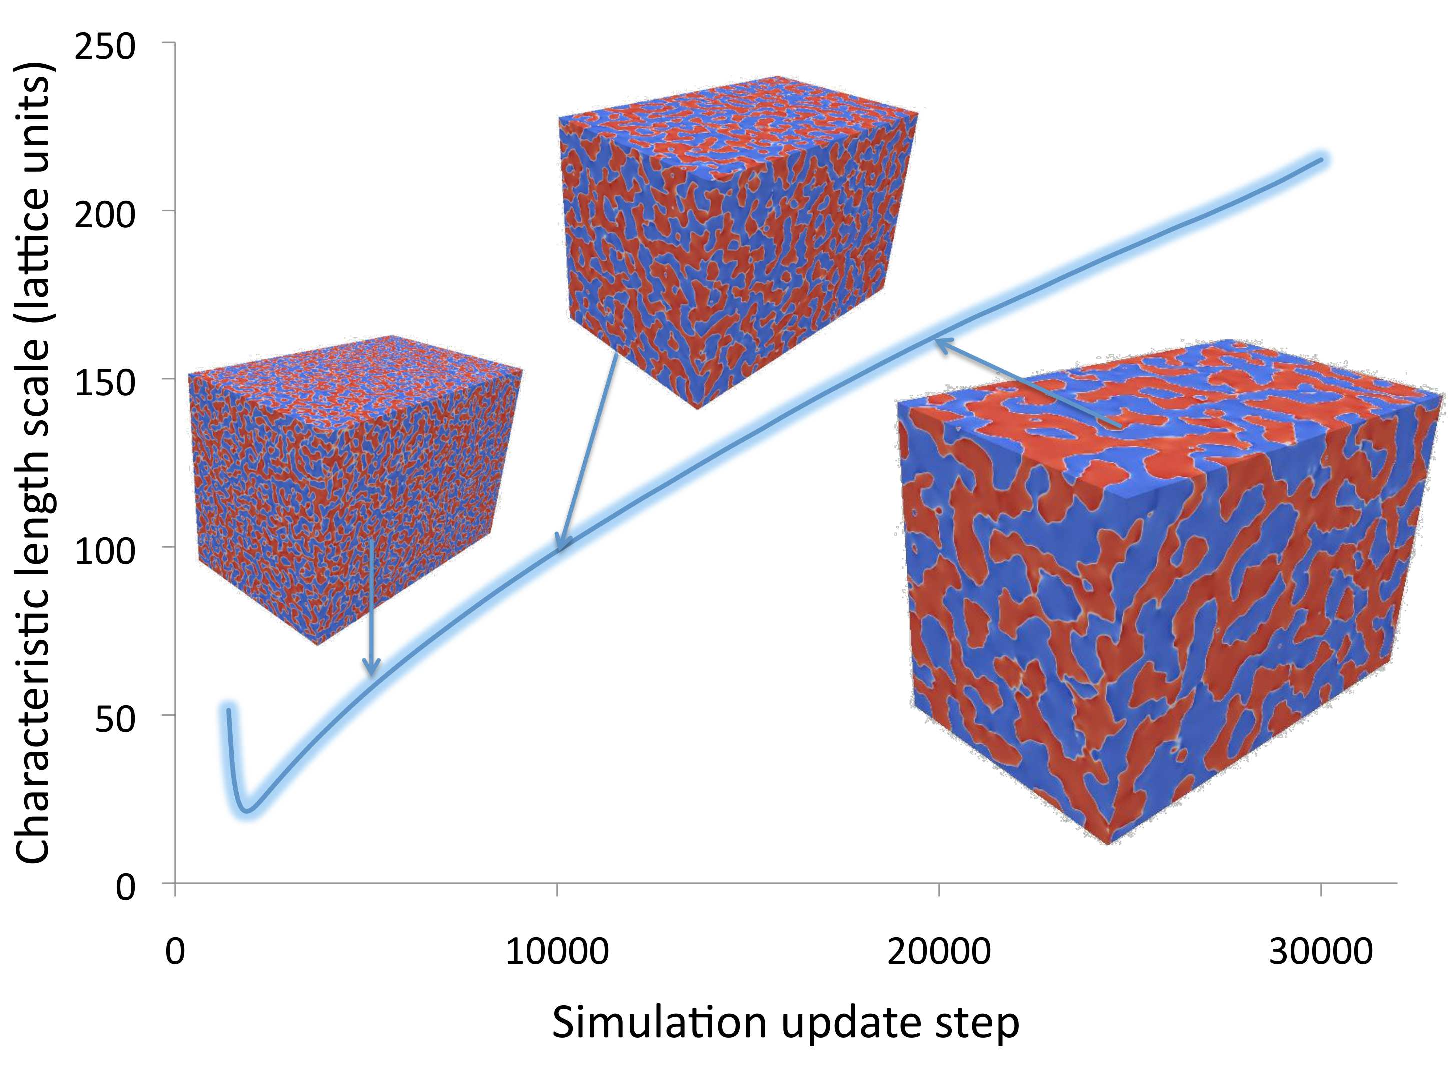
\includegraphics[width=10cm]{Chapters/chapter14/figures/length_scale}
\caption{The dependence of the characteristic length scale of a binary
  fluid mixture on the simulation timestep number. Superimposed are
  three snapshots showing increased mixture separation with time:
  these are obtained through the order parameter and each show one
  eighth of the total simulation size, which is $1548\times 1764\times 1568$. }\label{ch14:fig:length_scale}
\end{figure}  

\begin{figure}[!t]
\centering
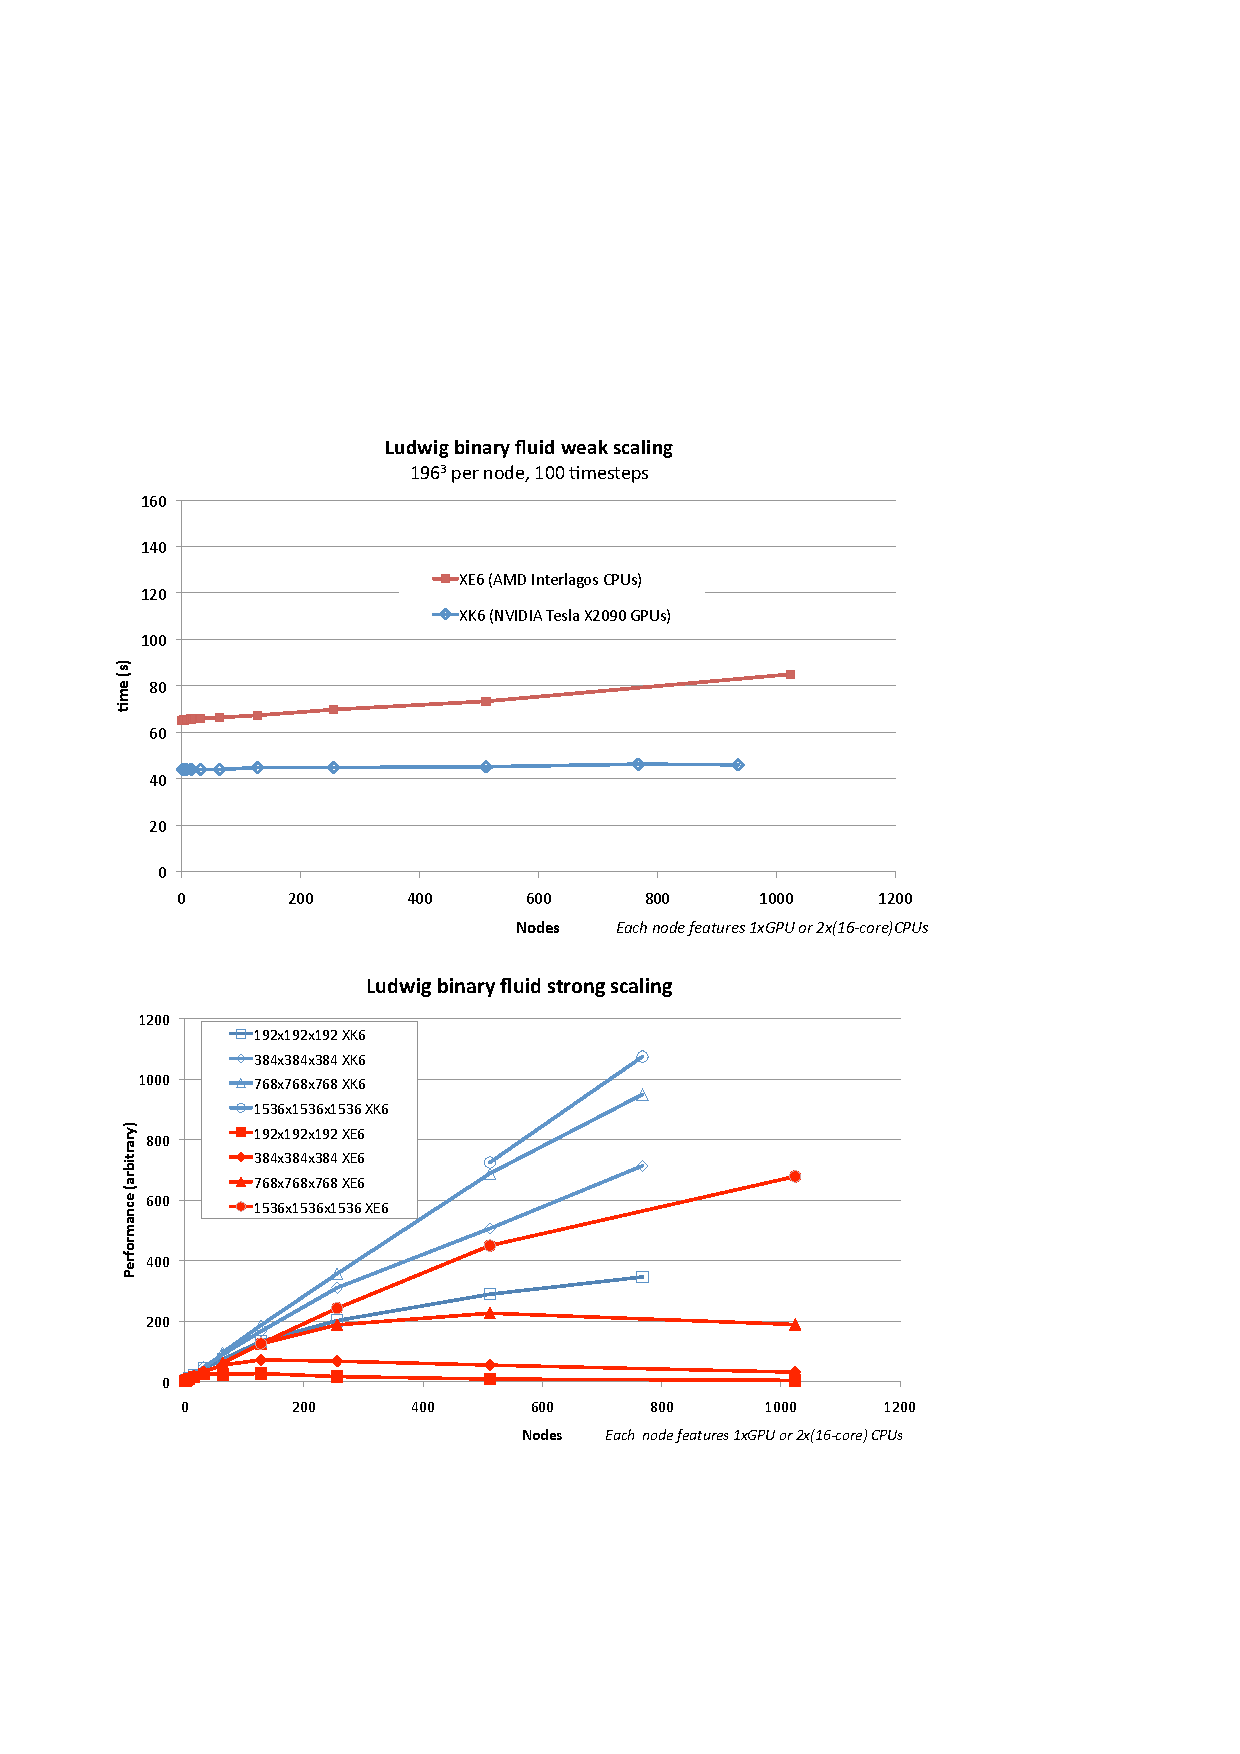
\includegraphics[width=10cm]{Chapters/chapter14/figures/two_graphs_ud}
\caption{The weak (top) and strong (bottom) scaling of Ludwig.  Closed
  shapes denote results using the traditional version run on the Cray
  XE6 (using two 16-core AMD Interlagos CPUs per node), while open
  shapes denote results using the GPU version on the Cray XK6 (using a
  single NVIDIA X2090 GPU per node). Top: the benchmark time is shown
  where the problem size per node is constant. Bottom: performance is
  shown where, for each of the four problem sizes presented, the
  results are scaled by the lattice volume, and all results are
  normalized by the same arbitrary constant.  }
\label{ch14:fig:scaling}
\end{figure}

The benchmark used involves the separation of an immiscible binary
fluid, where the characteristic length scale of fluid domains grows in
time in a well understood way \cite{kendon2001}. Figure
\ref{ch14:fig:length_scale} shows the characteristic length scale as a
function of time (both in LB units) for a system of size $1548\times
1764\times 1568$ run for around 12 hours on the Cray XK6 using 936
GPUs. The insets show a visualization of the fluid domains at
different times.  For the following comparisons we restrict our
benchmark runs to 100 timesteps: this is representative of the full
run.

The top of Figure \ref{ch14:fig:scaling} shows the benchmark time,
where the problem size is increased with the number of nodes. This
shows weak scaling: the time taken by a perfectly scaling code would
remain constant. The figure plots the time against the number of {\it
  nodes}: for the GPU version we utilize the one GPU per Cray XK6 node
whilst for the traditional version we fully utilize two 16-core CPUs
per Cray XE6 node, i.e. one GPU is compared with 32 CPU cores.  We use
a single MPI task per Cray XK6 node to host the GPU, and 32 MPI tasks
to fully utilize the CPUs in the Cray XE6 node.  Note that our CPU
version is highly optimised: in particular it has been tuned for
optimal utilisation of the SIMD vector units in each CPU core.
The new GPU version scales almost perfectly: the scaling advantage
over the CPU version is likely caused by the fact that the GPU version
has a factor of 32 less MPI tasks per node, hence communications
require a larger number of smaller data buffers. The performance
advantage of the GPU version ranges from a factor of around 1.5 to
around 1.8.  

We present a strong scaling comparison in the bottom of Figure
\ref{ch14:fig:scaling}, where we measure the performance (inverse
runtime) varying the number of nodes utilized (where we used up to 768
nodes), for several fixed problem sizes (where for each size we scale
results by the lattice volume to allow plotting on the same graph).
It can be seen that, for each of the four problem sizes, the GPU
adaptation on the Cray XK6 scales better (i.e.  the series are closer
to linearity) than the traditional version on the Cray XE6.  It can be
seen that ideal scaling is being approached by the larger problem
sizes.  The higher performance of the GPU version is manifested in the
larger gradients of the Cray XK6 series.

\section{Inclusion of Particles}\label{ch14:sec:particles}

\begin{figure}[t]
\centering
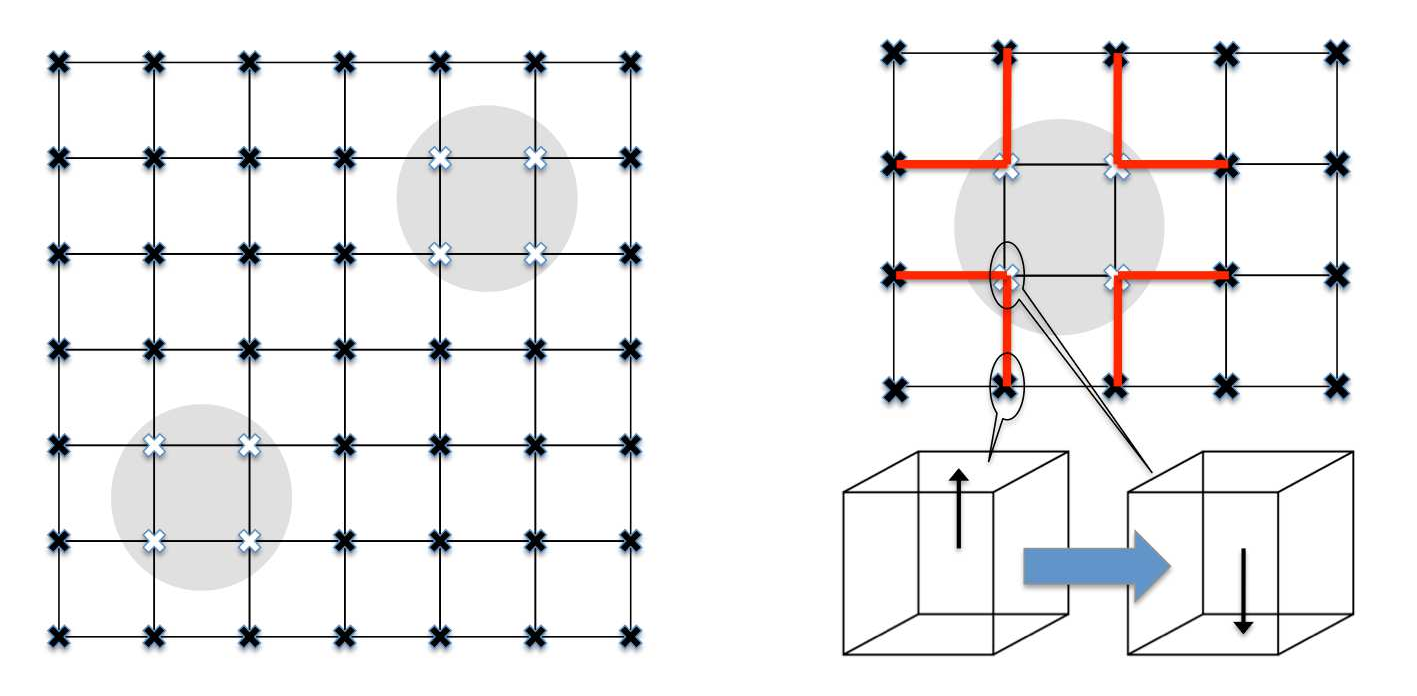
\includegraphics[width=10cm]{Chapters/chapter14/figures/bbl}
\caption{A 2D illustration of colloidal particles (grey circles)
  interacting with the lattice, where each lattice point is
  represented by a cross. Left: each particle spans multiple sites.
  Right: the particle-facing distribution components are moved inside
  the particle with the direction reversed, such that the ``bounce
  back'' will be completed when the fluid propagates.}
\label{ch14:fig:bbl}
\end{figure}


\begin{figure}[t]
\centering
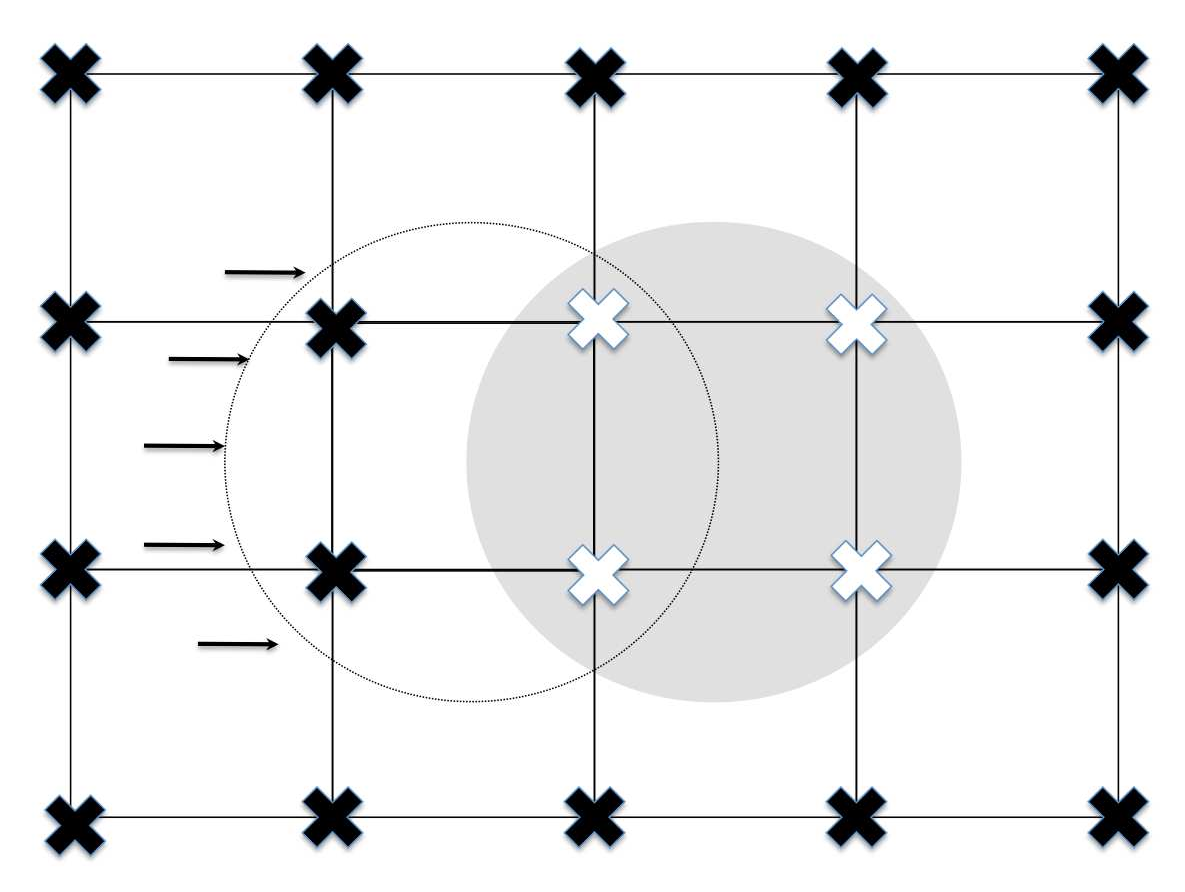
\includegraphics[width=6cm]{Chapters/chapter14/figures/particlemove}
\caption{A 2D illustration of a colloidal particle moving across the
    lattice. The old and new positions are represented by the open and
    filled circles respectively.}
\label{ch14:fig:particlemove}
\end{figure}

It is of interest, in many situations, to include colloidal particles
in the simulation **more from Kevin***. These are by represented by
moving spheres that interact with the fluid through transfer of
momenta: fluid coming into contact with a particle will bounce off it,
giving the particle a kick in the process. As illustrated on the left
of Figure \ref{ch14:fig:bbl} (which shows 2 dimensions only for
clarity - in practice, the particles will be represented by spheres on
a 3D lattice, and will be much larger relative to the lattice
spacing), typically each particle spans multiple lattice sites, and
therefore ``intercepts'' multiple inter-site links. Ludwig stores
particle information using nested linked lists: a list of particles,
each with a list of all the links intercepted by that particle (plus
other quantities). The fluid-particle interaction proceeds using the
so-called {\it bounce back on links} procedure during each timestep. As
illustrated in the right of Figure \ref{ch14:fig:bbl}, for each of the
intercepting links, those velocity components of the distribution that
face inwards to each particle are moved from the site
outside the particle to the site inside the particle, and
reversed in direction. This is done before the propagation stage,
which then propagates these same velocity components back out of the
particles: the velocity bounces back from the particles. The
momenta transfer from fluid to particles is also determined
from the distribution values.

A simplified schematic of the implementation on the CPU is as follows,
noting that multiplicative coefficients are required:
{\footnotesize
\begin{verbatim}
For each particle:
  For each link:
    Calculate coefficient
    Bounce back fluid using coefficient
    Update particle momentum
\end{verbatim}
}
This process is relatively inexpensive on the CPU, since the total
number of particles (and intercepted links) is always relatively
small, but it does require access to distribution data which we want
to keep resident on the GPU throughout the simulation. The overhead of
transferring the full distribution to the CPU and back every timestep
would be too high. But on the other hand, the full codebase required
to manage particles is quite complex and comprehensive: completely
porting it to the GPU, such that the particles effectively also remain
resident on the GPU, would be a large effort and would cause a major
diversion of CPU and GPU codebases. Further complications would arise
when running on multiple GPUs due to the fact that particles can move
between parallel subdomains. Our solution, which minimises overhead,
is to keep the particles resident on CPU, but offload only their interaction with the fluid to the GPU, as we describe below.
 
On the CPU, the code in the above listing can be restructured into
three distinct stages as (introducing arrays to temporrily store
indices and data):
{\footnotesize
\begin{verbatim}
1) For each particle, for each link:
     Store site and velocity indices associated with link
     Calculate and store coefficient
2) For each particle, for each link:
     Update velocity data using stored values
     Calculate and store particle momenta updates
3) For each particle, for each link:
     Update particle momentum using stored values
\end{verbatim}
}
Stage 2 is only one that that accesses fluid data: this can therefore
be moved to the GPU, while stages 1 and 3 remain on the CPU. Stage 2
therefore becomes, for the GPU implementation
{\footnotesize
\begin{verbatim}
Transfer coefficient and link index arrays to GPU
Run CUDA kernel:
  Update fluid data using coefficient and link index arrays
  Calculate and store particle momenta updates from fluid data
Transfer particle momenta updates array back to CPU
\end{verbatim}
}
Since the total number of links involves is relatively small, these
partial data transfers have minimal overhead.  A complication arises
due to the fact that the particles move through the lattice, albeit
relatively slowly, and therefore the list of links that they intercept
occasionally changes (see Figure \ref{ch14:fig:particlemove}).  When a
particle moves off a lattice site, the fluid on that site must be
reconstructed. Similarly, the fluid on the newly obstructed site must
be removed. For the same reasons given above, we want to avoid moving
all the code dealing with this complication to the GPU, whilst
minimising overheads. Since, on any one timestep, the number of
lattice sites affected is relatively low, we implement functionality
to perform partial data transfers of the distribution. Only those
sites affected are packed into a buffer on the GPU, transferred to the
CPU and unpacked into the CPU version of the distribution. Then, the
existing code can be used to update those affected sites, before the
reverse partial data transfer is performed to update the GPU version
of data.

Our methods for managing particles allow us to exploit the GPU for the
intensive fluid simulation whilst maintaining the complex code
required to manage particles on the CPU, with overheads minimised
through only transferring those small subsets of data corresponding to
the points of interaction.



\section{Summary}

The \textit{Ludwig} LB application, which specializes
in complex fluid problems, has undergone the developments required to
efficiently use large-scale parallel GPU accelerated supercomputers.
The new functionality augments the original code, such that the
package now supports both traditional CPU-based and GPU-accelerated
systems. 

Through use of the NVIDIA CUDA programming language the computational
kernels in the Ludwig timestep were offloaded to the GPU, including
not just those responsible for the majority of the compute time but
any that accessed the main data structures, to allow data to be kept
resident on the GPU and avoid expensive data transfers. We described
steps taken to optimise the performance on the GPU architecture through
reducing off-chip memory accesses and including the restructuring of
data layout in memory to ensure the available memory bandwidth was
fully exploited.

A new halo-exchange communication phase for the code was developed to
allow efficient parallel scaling to many GPUs. The traditional version
relies on MPI datatype functionality for CPU to CPU communication; we
have explicitly written buffer packing/unpacking and transfer
operations to for GPU to GPU data exchange, staged through the host
CPUs. This includes the filtering of velocity components to only
transfer those required in a specific direction, hence reducing the
overall volume of data transferred. We used CUDA stream functionality
to overlap separate stages within the communication phase, and reduce
the overall communication time. The effect was measured to be more
profound for smaller local system sizes, i.e. it is especially useful
in aiding strong scaling.

We compared performance, for a binary fluid benchmark, of the new GPU
adaptation using up to 936 GPUs in parallel on prototype Cray XK6 GPU
accelerated hardware, comparing to runs on the counterpart CPU based
Cray XE6 using the (optimized) traditional version. We compare on a
node-by-node basis, i.e. each GPU against 2 CPUs (or 32 cores),
ensuring full utilization of each CPU.  The performance of the GPU
version on the Cray XK6 version is around a factor of 1.5-1.8 better
than the traditional version on the Cray XE6, depending on how many
nodes is used in the comparison. The weak scaling of the GPU version
is excellent up to the 936 GPUs tested. The scaling advantage over the
traditional version is likely due to the fact that we have a factor of
32 less MPI processes per node. The ability to strong scale depends on
the physical system size; as the size increases ideal scaling is
approached. The strong scaling of the GPU version is better than that
for the CPU version, for each of the sizes tested.

We described work to enable colloidal particles in the simulation with
minimal overhead. We implemented these in such a way that we avoid a
major diversion of the CPU and GPU codebases, whilst minimising data
transfers between the CPU and GPU at each timestep. We keep the
majority of the (relatively inexpensive) particle related code on the
CPU, while offloading only those parts responsible for the interaction
with the fluid to the GPU (where the fluid data resides).

Our resulting package is able to exploit the largest of GPU
accelerated architectures to address a wide range of complex problems.



%\section{Introduction}
%% no \IEEEPARstart
%This demo file is intended to serve as a ``starter file''
%for IEEE conference papers produced under \LaTeX\ using
%IEEEtran.cls version 1.7 and later.
%% You must have at least 2 lines in the paragraph with the drop letter
%% (should never be an issue)
%I wish you the best of success.

%\hfill mds
 
%\hfill January 11, 2007

%\subsection{Subsection Heading Here}
%Subsection text here.


%\subsubsection{Subsubsection Heading Here}
%Subsubsection text here.


% An example of a floating figure using the graphicx package.
% Note that \label must occur AFTER (or within) \caption.
% For figures, \caption should occur after the \includegraphics.
% Note that IEEEtran v1.7 and later has special internal code that
% is designed to preserve the operation of \label within \caption
% even when the captionsoff option is in effect. However, because
% of issues like this, it may be the safest practice to put all your
% \label just after \caption rather than within \caption{}.
%
% Reminder: the "draftcls" or "draftclsnofoot", not "draft", class
% option should be used if it is desired that the figures are to be
% displayed while in draft mode.
%
%\begin{figure}[!t]
%\centering
%\includegraphics[width=2.5in]{myfigure}
% where an .eps filename suffix will be assumed under latex, 
% and a .pdf suffix will be assumed for pdflatex; or what has been declared
% via \DeclareGraphicsExtensions.
%\caption{Simulation Results}
%\label{fig_sim}
%\end{figure}

% Note that IEEE typically puts floats only at the top, even when this
% results in a large percentage of a column being occupied by floats.


% An example of a double column floating figure using two subfigures.
% (The subfig.sty package must be loaded for this to work.)
% The subfigure \label commands are set within each subfloat command, the
% \label for the overall figure must come after \caption.
% \hfil must be used as a separator to get equal spacing.
% The subfigure.sty package works much the same way, except \subfigure is
% used instead of \subfloat.
%
%\begin{figure*}[!t]
%\centerline{\subfloat[Case I]\includegraphics[width=2.5in]{subfigcase1}%
%\label{fig_first_case}}
%\hfil
%\subfloat[Case II]{\includegraphics[width=2.5in]{subfigcase2}%
%\label{fig_second_case}}}
%\caption{Simulation results}
%\label{fig_sim}
%\end{figure*}
%
% Note that often IEEE papers with subfigures do not employ subfigure
% captions (using the optional argument to \subfloat), but instead will
% reference/describe all of them (a), (b), etc., within the main caption.


% An example of a floating table. Note that, for IEEE style tables, the 
% \caption command should come BEFORE the table. Table text will default to
% \footnotesize as IEEE normally uses this smaller font for tables.
% The \label must come after \caption as always.
%
%\begin{table}[!t]
%% increase table row spacing, adjust to taste
%\renewcommand{\arraystretch}{1.3}
% if using array.sty, it might be a good idea to tweak the value of
% \extrarowheight as needed to properly center the text within the cells
%\caption{An Example of a Table}
%\label{table_example}
%\centering
%% Some packages, such as MDW tools, offer better commands for making tables
%% than the plain LaTeX2e tabular which is used here.
%\begin{tabular}{|c||c|}
%\hline
%One & Two\\
%\hline
%Three & Four\\
%\hline
%\end{tabular}
%\end{table}


% Note that IEEE does not put floats in the very first column - or typically
% anywhere on the first page for that matter. Also, in-text middle ("here")
% positioning is not used. Most IEEE journals/conferences use top floats
% exclusively. Note that, LaTeX2e, unlike IEEE journals/conferences, places
% footnotes above bottom floats. This can be corrected via the \fnbelowfloat
% command of the stfloats package.


% conference papers do not normally have an appendix


% use section* for acknowledgement
\section*{Acknowledgments}
This work has been supported by the CRESTA project that has received
funding from the European Community's Seventh Framework Programme
(ICT-2011.9.13) under Grant Agreement no. 287703. 


% trigger a \newpage just before the given reference
% number - used to balance the columns on the last page
% adjust value as needed - may need to be readjusted if
% the document is modified later
%\IEEEtriggeratref{8}
% The "triggered" command can be changed if desired:
%\IEEEtriggercmd{\enlargethispage{-5in}}

% references section

% can use a bibliography generated by BibTeX as a .bbl file
% BibTeX documentation can be easily obtained at:
% http://www.ctan.org/tex-archive/biblio/bibtex/contrib/doc/
% The IEEEtran BibTeX style support page is at:
% http://www.michaelshell.org/tex/ieeetran/bibtex/
%\bibliographystyle{IEEEtran}
% argument is your BibTeX string definitions and bibliography database(s)
%\bibliography{IEEEabrv,../bib/paper}
%
% <OR> manually copy in the resultant .bbl file
% set second argument of \begin to the number of references
% (used to reserve space for the reference number labels box)


\begin{thebibliography}{1}

%\bibitem{IEEEhowto:kopka}
%H.~Kopka and P.~W. Daly, \emph{A Guide to \LaTeX}, 3rd~ed.\hskip 1em plus
%  0.5em minus 0.4em\relax Harlow, England: Addison-Wesley, 1999.



\bibitem{succi-book}
S. Succi, \textit{The lattice Boltzmann equation and beyond},
Oxford University Press, Oxford, 2001.

\bibitem{mpi-standard}
Message Passing Interface Forum, http://www.mpi-forum.org 

\bibitem{desplat}
Desplat, J.-C., I. Pagonabarraga, and P. Bladon,
\textit{LUDWIG: A parallel lattice-Boltzmann code for complex fluids}.
Comput. Phys. Comms., \textbf{134}, 273, 2001.

\bibitem{aidun2010}
C.K. Aidun and J.R. Clausen,
\textit{Lattice Botlzmann method for complex flows},
Ann. Rev. Fluid Mech., \textbf{42} 439--472 (2010).

\bibitem{bray1994}
A.J. Bray,
\textit{Theory of phase-ordering kinetics},
Adv. Phys., \textbf{43} 357--459 (1994).

\bibitem{kendon2001}
V.M. Kendon, M.E. Cates, I. Pangonabarraga, J.-C. Desplat, and P. Bladon,
\textit{Inertial effects in the three-dimensional spinodal decomposition of a
symmetric binary fluid mixture; a lattice Boltzmann study},
J. Fluid Mech., \textbf{440}, 147--203 (2001).

\bibitem{swift1996}
M.R. Swift, E. Orlandini, W.R. Osborn, and J.M. Yeomans,
\textit{Lattice Boltzmann simulations of liquid-gas and binary
fluid systems},
Phys. Rev. E, \textbf{54}, 5041--5052 (1996).


\bibitem{stratford-jsp2005}
K. Stratford, R. Adhikari, I. Pagonabarraga, and J.-C. Desplat,
\textit{Lattice Boltzmann for Binary Fluids with Suspended Colloids},
J. Stat. Phys. \textbf{121}, 163 (2005).

\bibitem{xe6}
Cray XE6 Product Brochure, available from http://www.cray.com/Products/XE/Resources.aspx (2010)

\bibitem{hector} HECToR home page, http://www.hector.ac.uk

\bibitem{xk6}
Cray XK6 Product Brochure, available from http://www.cray.com/Products/XK6/XK6.aspx (2011)


%\bibitem{wei2004}
%X. Wei, W. Li, K. M\"uller, and A.E. Kaufman,
%\textit{The lattice Blotzmann method for simulating gaseous phenomena},
%IEEE Transactions on Visualization and Computer Graphics,
%\textbf{10}, 164--176 (2004).
%% Apparently first LB via GPU; a serious contribution using single fluid
%%d3q19 single relaxation time.

%\bibitem{zhu2006}
%H. Zhu, X. Liu, Y. Liu, and E. Wu,
%\textit{Simulation of miscible binary mixtures based on lattice Boltzmann method},
%Comp. Anim. Virtual Worlds, \textbf{17}, 403--410 (2006).
%% Single relaxation (MRT mentioned) time d3q19 apparently sound although
%%not a lot of detail. Pre-cuda so graphics code.

%\bibitem{zhao2007}
%Y. Zhao,
%\textit{Lattice Boltzmann based PDE solver on the GPU},
%Visual Comput., doi 10.1007/s00371-0070191-y (2007).

%\bibitem{toelke}
%J. T\"olke,
%\textit{Implementation of a lattice Boltzmann kernel using the Compute Unified
%Device Architecture developed by NVIDIA},
%Comput. Visual. Sci. doi:10.1007/s00791-008-0120-2 (2008).

%\bibitem{fan2004}
%Z. Fan, F. Qiu, A. Kaufman, and S. Yoakum-Stover,
%\textit{GPU cluster for high performance computing},
%Proceedings of ACM/IEEE Supercomputing Conference, pp. 47--59,
%IEEE Computer Society Press, Pittsburgh, PA (2004).

%\bibitem{myre2011}
%J. Myre, S.D.C. Walsh, D. Lilja, and M.O. Saar,
%\textit{Performance analysis of single-phase, multiphase, and multicomponent
%lattice Boltzmann fluid flow simulations on GPU clusters},
%Concurrency Computat.: Pract. Exper., \textbf{23}, 332--350 (2011).

%\bibitem{obrecht2011}
%C. Obrecht, F. Kuznik, B. Tourancheau, and J.-J. Roux,
%\textit{Multi-GPU implementation of the lattice Boltzmann method},
%Comput. Math. with Applications,
%doi:10.1016/j.camwa.2011.02.020 (2011).

%\bibitem{bernaschi2010}
%M. Bernaschi, M. Fatica, S. Melchionna, S. Succi, and E. Kaxiras,
%\textit{A flexible high-performance lattice Boltzmann GPU code for the
%simulations of fluid flow in complex geometries},
%Concurrency Computat.: Pract. Exper., \textbf{22}, 1--14 (2010).

%\bibitem{xian2011}
%W. Xian and A. Takayuki,
%\textit{Multi-GPU performance of incompressible flow computation by
%lattice Boltzmann method on GPU cluster},
%Parallel Comput., doi:10.1016/j.parco.2011.02.007 (2011). 







%\bibitem{simd} Intel AVX: New Frontiers in Performance Improvements and Energy Efficiency, Intel article, http://software.intel.com/en-us/articles (2009)


%\bibitem{amd} AMD 6200 series home page  
%http://www.amd.com/us/products/server/
%processors/6000-series-platform/6200/Pages/6200-series-processors.aspx (accessed April 2012)

%\bibitem{nvidia} NVIDIA Tesla home page, http://www.nvidia.com/object/
%tesla\_computing\_solutions.html (accessed April 2012)


%\bibitem{titan} \textit{ORNL awards contract to Cray for Titan supercomputer}, Oak Ridge National Laboratory Press Release mr20111011-00, http://www.ornl.gov/info/press\_releases/ (2011)

\end{thebibliography}




% that's all folks
\end{document}


